% !TeX root = exercises_main.tex
\section*{Task 4: Fish Farming}

\begin{enumerate}[label=\alph*)]
    \item\label{item:task4a} The population of fish $P(t)$ in a pond can be described by the following ODE
    \begin{equation}\label{eq:fish}
    \frac{d}{dt}P(t) = rP(t)\left(1 - \frac{P(t)}{C}\right)
    \end{equation}
    The constants $r$ and $C$ specify the growth rate and maximum capacity of the pond. \\\\
    \textbf{Subtask:} \\
    Use IFDIFF to solve the ODE on the time interval $I = [0, 5]$ with initial conditions $P(0) = 0.1$. \\
    Set the constants as $r = 2$ and $C = 1$ directly in the RHS (do not pass them as parameters). \\
    Plot the solution. What is the maximum size of the population? When does the population grow fastest? \\ \\
    \textbf{Steps:}
    \begin{enumerate}[label=\arabic*.]
        \item Implement the RHS in the file \texttt{rhsTask4.m} as described in \cref{eq:fish}. Remember to set the constants $r$ and $C$ directly in the RHS.
        \item Set the integration time span and initial conditions in the file \texttt{runTask4.m}. Ignore the parameters for now.
        \item Use IFDIFF's \lstinline|prepareDatahandleForIntegration| function to prepare the RHS for integration. Don't forget to include the integrator and its options.
        \item Use IFDIFF's \lstinline|solveODE| function to solve the initial value problem.
        \item Use the provided function \lstinline|plotPopulation(solution)| to plot your solution.
    \end{enumerate}
    \textbf{Hints:}
    \begin{itemize}
        \item Check the appendix for a reminder on how to formulate and solve an ODE using IFDIFF.
    \end{itemize}
    \textbf{Reference plot:}
    \begin{figure}[H]
        \centering
        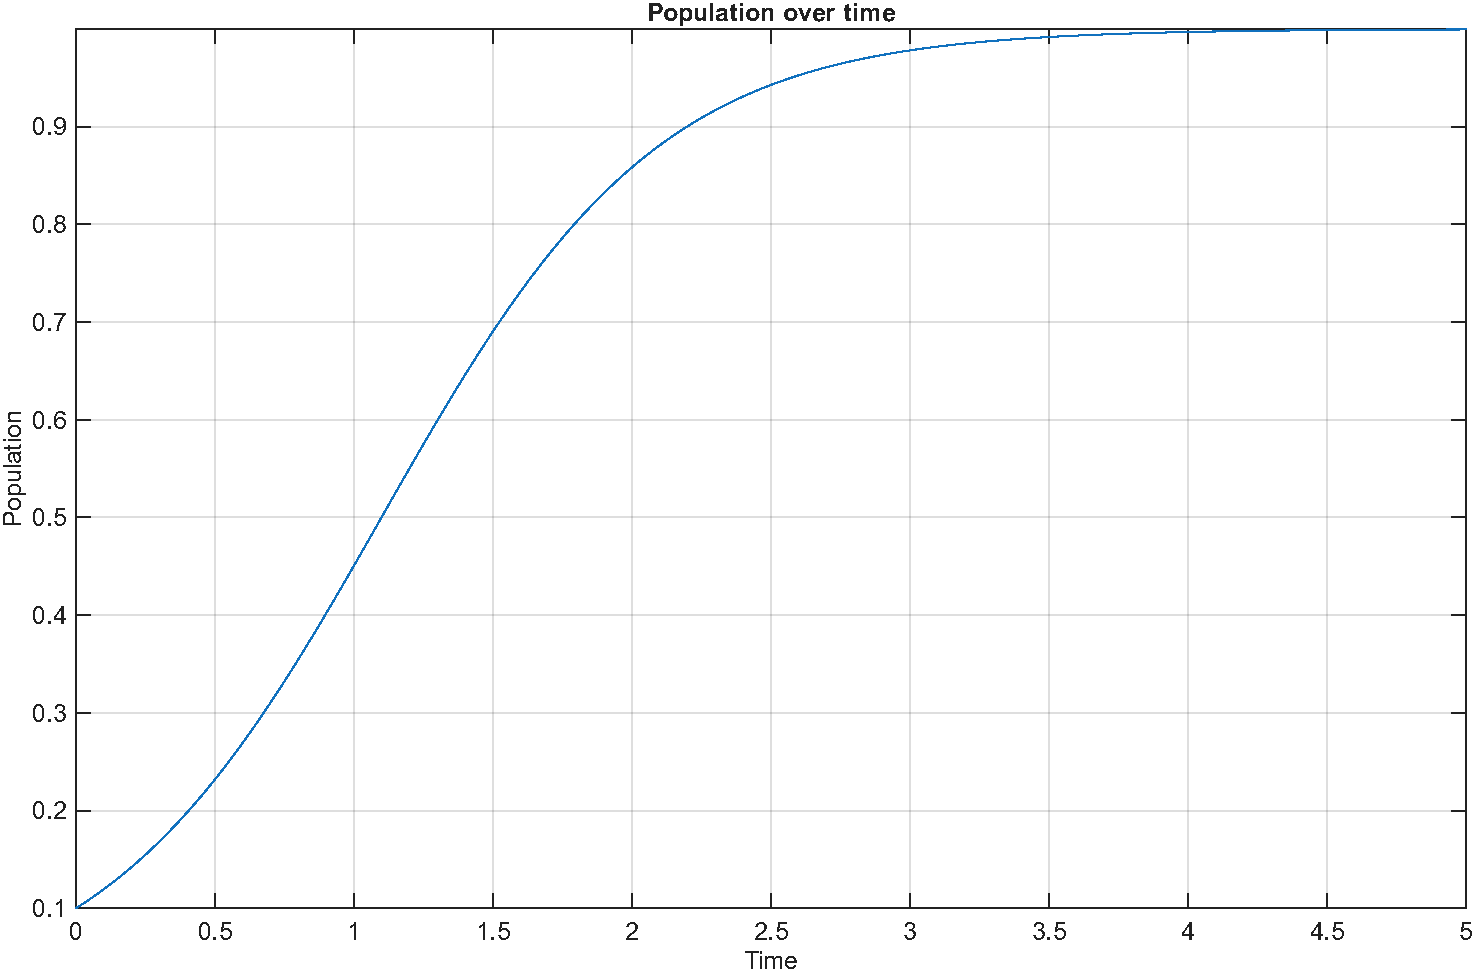
\includegraphics[width=\textwidth]{Plots/task4a}
        \caption{Population plot for subtask 4a)}
    \end{figure}

    \item The population of fish will now be harvested automatically according to the following rule:\\
    Whenever the population $P(t)$ would exceed a threshold $T \in [0, C]$, a proportion of the current population will be extracted from the pond and added to the harvest $H(t)$ according to the harvest ratio $\alpha \in [0, 1]$.

    This new system can be described by the following ODE
    \begin{equation}\label{eq:fish_harvest}
        \frac{d}{dt}\begin{bmatrix}P(t) \\ H(t)\end{bmatrix} = \begin{bmatrix}rP(t)\left(1 - \frac{P(t)}{C}\right) \\ 0\end{bmatrix}
    \end{equation}
    with state jumps
    \begin{equation}\label{eq:fish_jump}
        \begin{bmatrix}P(t^+) \\ H(t^+)\end{bmatrix} = \begin{bmatrix}P(t^-) \\ H(t^-)\end{bmatrix} +  \begin{bmatrix}-\alpha P(t^-) \\ \phantom{-}\alpha P(t^-)\end{bmatrix}, \quad P(t^-) = T
    \end{equation}

    \textbf{Subtask:} \\
    Use IFDIFF to solve the new system for the same constants and initial conditions as in subtask \ref{item:task4a} and $H(0) = 0$. \\
    Make sure to pass $p = (T, \alpha)$ as parameters to your RHS (do not set them directly in the RHS). \\
    Plot the solution. What is the maximum size of the population now? Play around with different parameters. \\ \\
    \textbf{Steps:}
    \begin{enumerate}[label=\arabic*.]
        \item Extend your RHS from subtask \ref{item:task4a} in the file \texttt{rhsTask4.m}. Split the state vector into two components and compute the derivatives as described in \cref{eq:fish_harvest}. \\
        Use the functions \lstinline|ifdiff_jumpif(condition, direction)| and \lstinline|ifdiff_update(jump)| to implement the state jump as described in \cref{eq:fish_jump}. \\
        Make sure that the components of your state and parameter vectors are defined in the same way as in the exercise sheet, i.e.~$y = (P, H)^T$ and $p = (T, \alpha)$.
        \item Add the second component to your initial conditions state vector in the file \texttt{runTask4.m}.
        \item Use your code from subtask \ref{item:task4a} to solve the new system and plot the solution. Try out different values for $T$ and $\alpha$.
    \end{enumerate}
    \textbf{Hints:}
    \begin{itemize}
        \item Check the appendix for a reminder on how to formulate state jumps in a RHS using IFDIFF.
        \item Verify that your states and parameters are defined correctly: $y = (P, H)^T$ and $p = (T, \alpha)$.
        \item Don't forget to include the second component of the state vector in your initial conditions.
        \item Make sure that your jump condition and direction match, i.e.~the direction should be 1 if the jump is triggered when the condition goes from negative to positive and -1 for the other way around.
    \end{itemize}
    \textbf{Reference plot:}
    \begin{figure}[H]
        \centering
        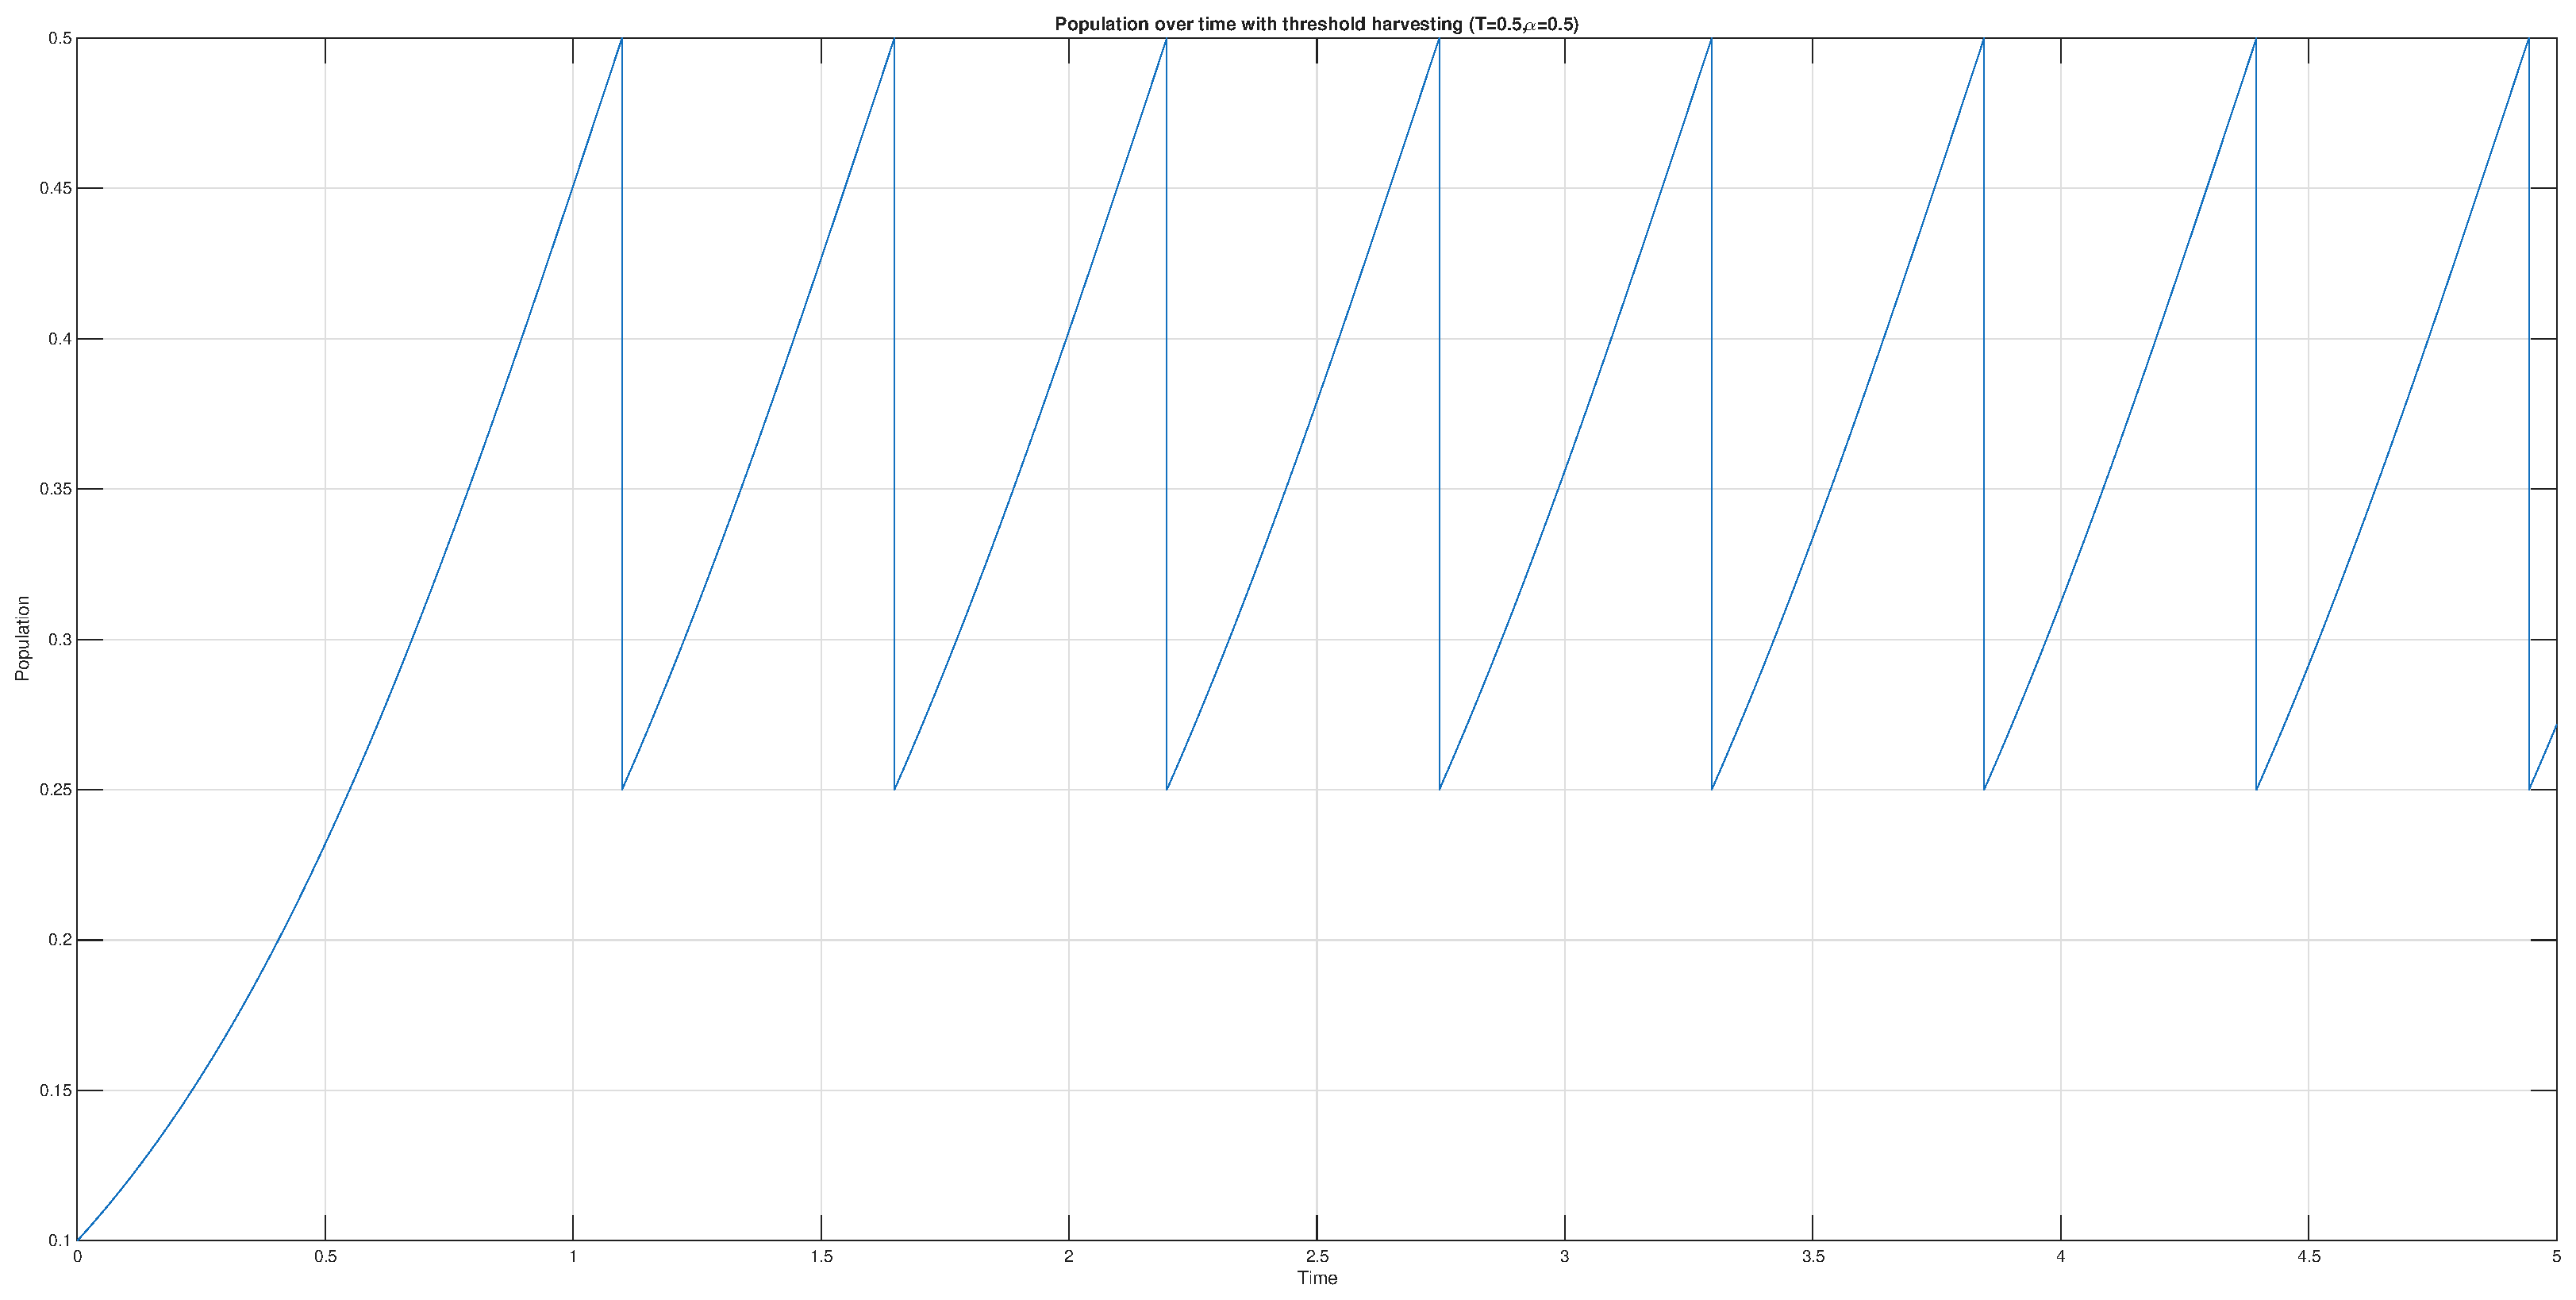
\includegraphics[width=\textwidth]{Plots/task4b}
        \caption{Population plot for subtask 4b)}
    \end{figure}

    \item \label{item:task4c} We now want to examine how the solution behaves depending on the parameters $T$ and $\alpha$. \\ \\
    \textbf{Subtask:} \\
    Discretize the parameter space $p = (T, \alpha) \in [0, C] \times [0, 1]$ as a 2D grid. \\
    Use IFDIFF to compute a solution for each parameter in the grid and plot the results. \\
    Explain the behavior at the grid boundaries, i.e.~for $T = 0,\: T = C$ and $\alpha = 0, \:\alpha = 1$. \\ \\
    \textbf{Steps:}
    \begin{enumerate}[label=\arabic*.]
       \item Implement the anonymous function \lstinline|solutionFunc = @(p) ...| in the file \texttt{runTask4.m}, which should take a parameter vector and use IFDIFF's \lstinline|solveODE| function to compute a solution for the given parameter.
       \item Use the provided function \lstinline|solutionGrid = solveOnGrid(solutionFunc)| to generate a solution for each parameter in the discretization grid.
       \item Use the provided function \lstinline|plotPopulationGrid(solutionGrid)| to plot your solutions on a grid.
    \end{enumerate}
    \textbf{Hints:}
    \begin{itemize}
       \item You can define an anonymous function in MATLAB using the \lstinline|@| operator followed by parantheses \lstinline|()| containing the arguments of the function and finally an expression which defines the return value. Note that anonymous functions can also store copies of variables defined outside of the function and use them to compute their return value.
       \begin{lstlisting}
c = 5;
func = @(a, b) a + b + c;
func(2, 3) == 10 % true
        \end{lstlisting}
        The anonymous function \lstinline|func| defined above takes two numbers \lstinline|a| and \lstinline|b| and returns \lstinline|a + b + 5|.
    \end{itemize}
    \textbf{Reference plot:}
    \begin{figure}[H]
        \centering
        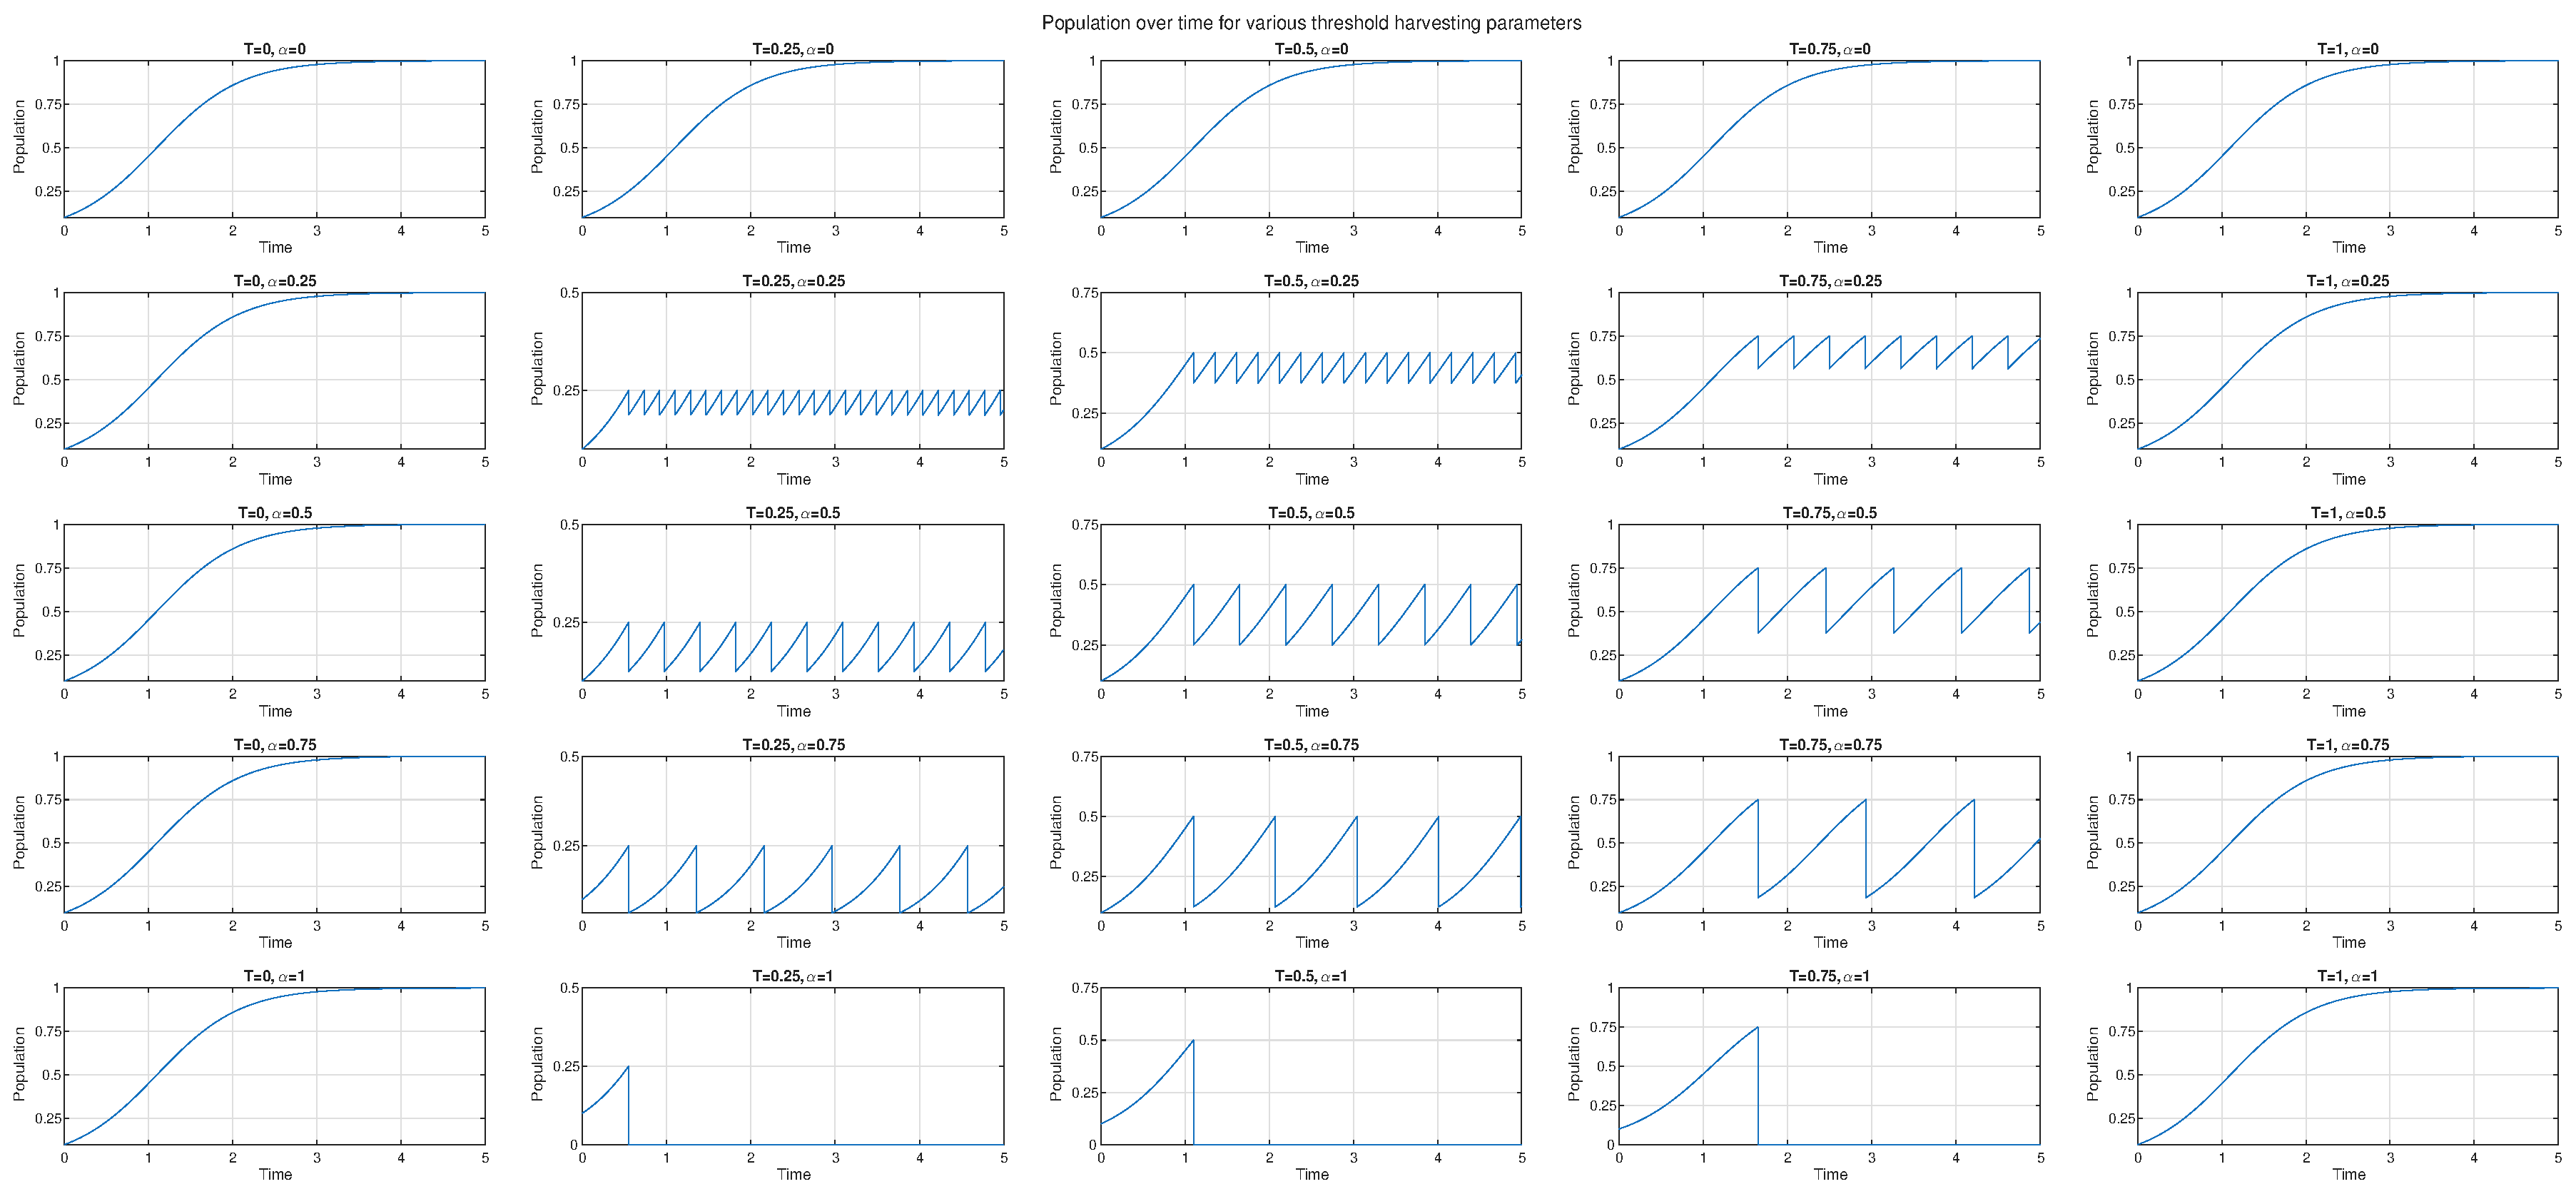
\includegraphics[width=\textwidth]{Plots/task4c}
        \caption{Population grid plot for subtask 4c)}
    \end{figure}

    \item The total amount of fish produced over the time interval $I = [0, 5]$ is given by the objective function
    \begin{equation}\label{eq:fish_objective}
       F(T, \alpha) = P(5; T, \alpha) + H(5; T, \alpha)
    \end{equation}
    where $P(t; T, \alpha)$ and $H(t; T, \alpha)$ denote the solution of the system given by \cref{eq:fish_harvest} and \cref{eq:fish_jump} with parameters $T$ and $\alpha$ at time point $t$. \\ \\
    \textbf{Subtask:} \\
    Compute the objective function $F$ on a parameter grid using the solutions obtained from subtask \ref{item:task4c}.\\
    Plot the result. Explain the behavior at the grid boundaries. Which combination of parameters on the grid maximizes $F$? \\ \\
    \textbf{Steps:}
    \begin{enumerate}[label=\arabic*.]
       \item Implement the anonymous function \lstinline|objectiveFunc = @(solution) ...| in the file \texttt{runTask4.m}, which should take a solution and return the value of the objective function $F$ for the given solution as described in \cref{eq:fish_objective}.
       \item Use the provided code \lstinline|objectiveGrid = arrayfun(objectiveFunc, solutionGrid)| to apply your objective function to each solution in the grid.
       \item Use the provided function \lstinline|plotObjective(solutionGrid, objectiveGrid)| to plot your objective function as a 3D surface plot.
    \end{enumerate}
    \textbf{Hints:}
    \begin{itemize}
       \item A solution struct (as returned by MATLAB integrators and IFDIFF) stores the timepoints at which the solution was computed in ascending order as a vector in the field \lstinline|solution.x|. The field \lstinline|solution.y(i, j)| stores the i-th component of the solution state vector at the timepoint \lstinline|solution.x(j)|. You can access the state vector of the solution at the final timepoint in the integration time interval using \lstinline|solution.y(:, end)|.
    \end{itemize}
    \textbf{Reference plot:}
    \begin{figure}[H]
        \centering
        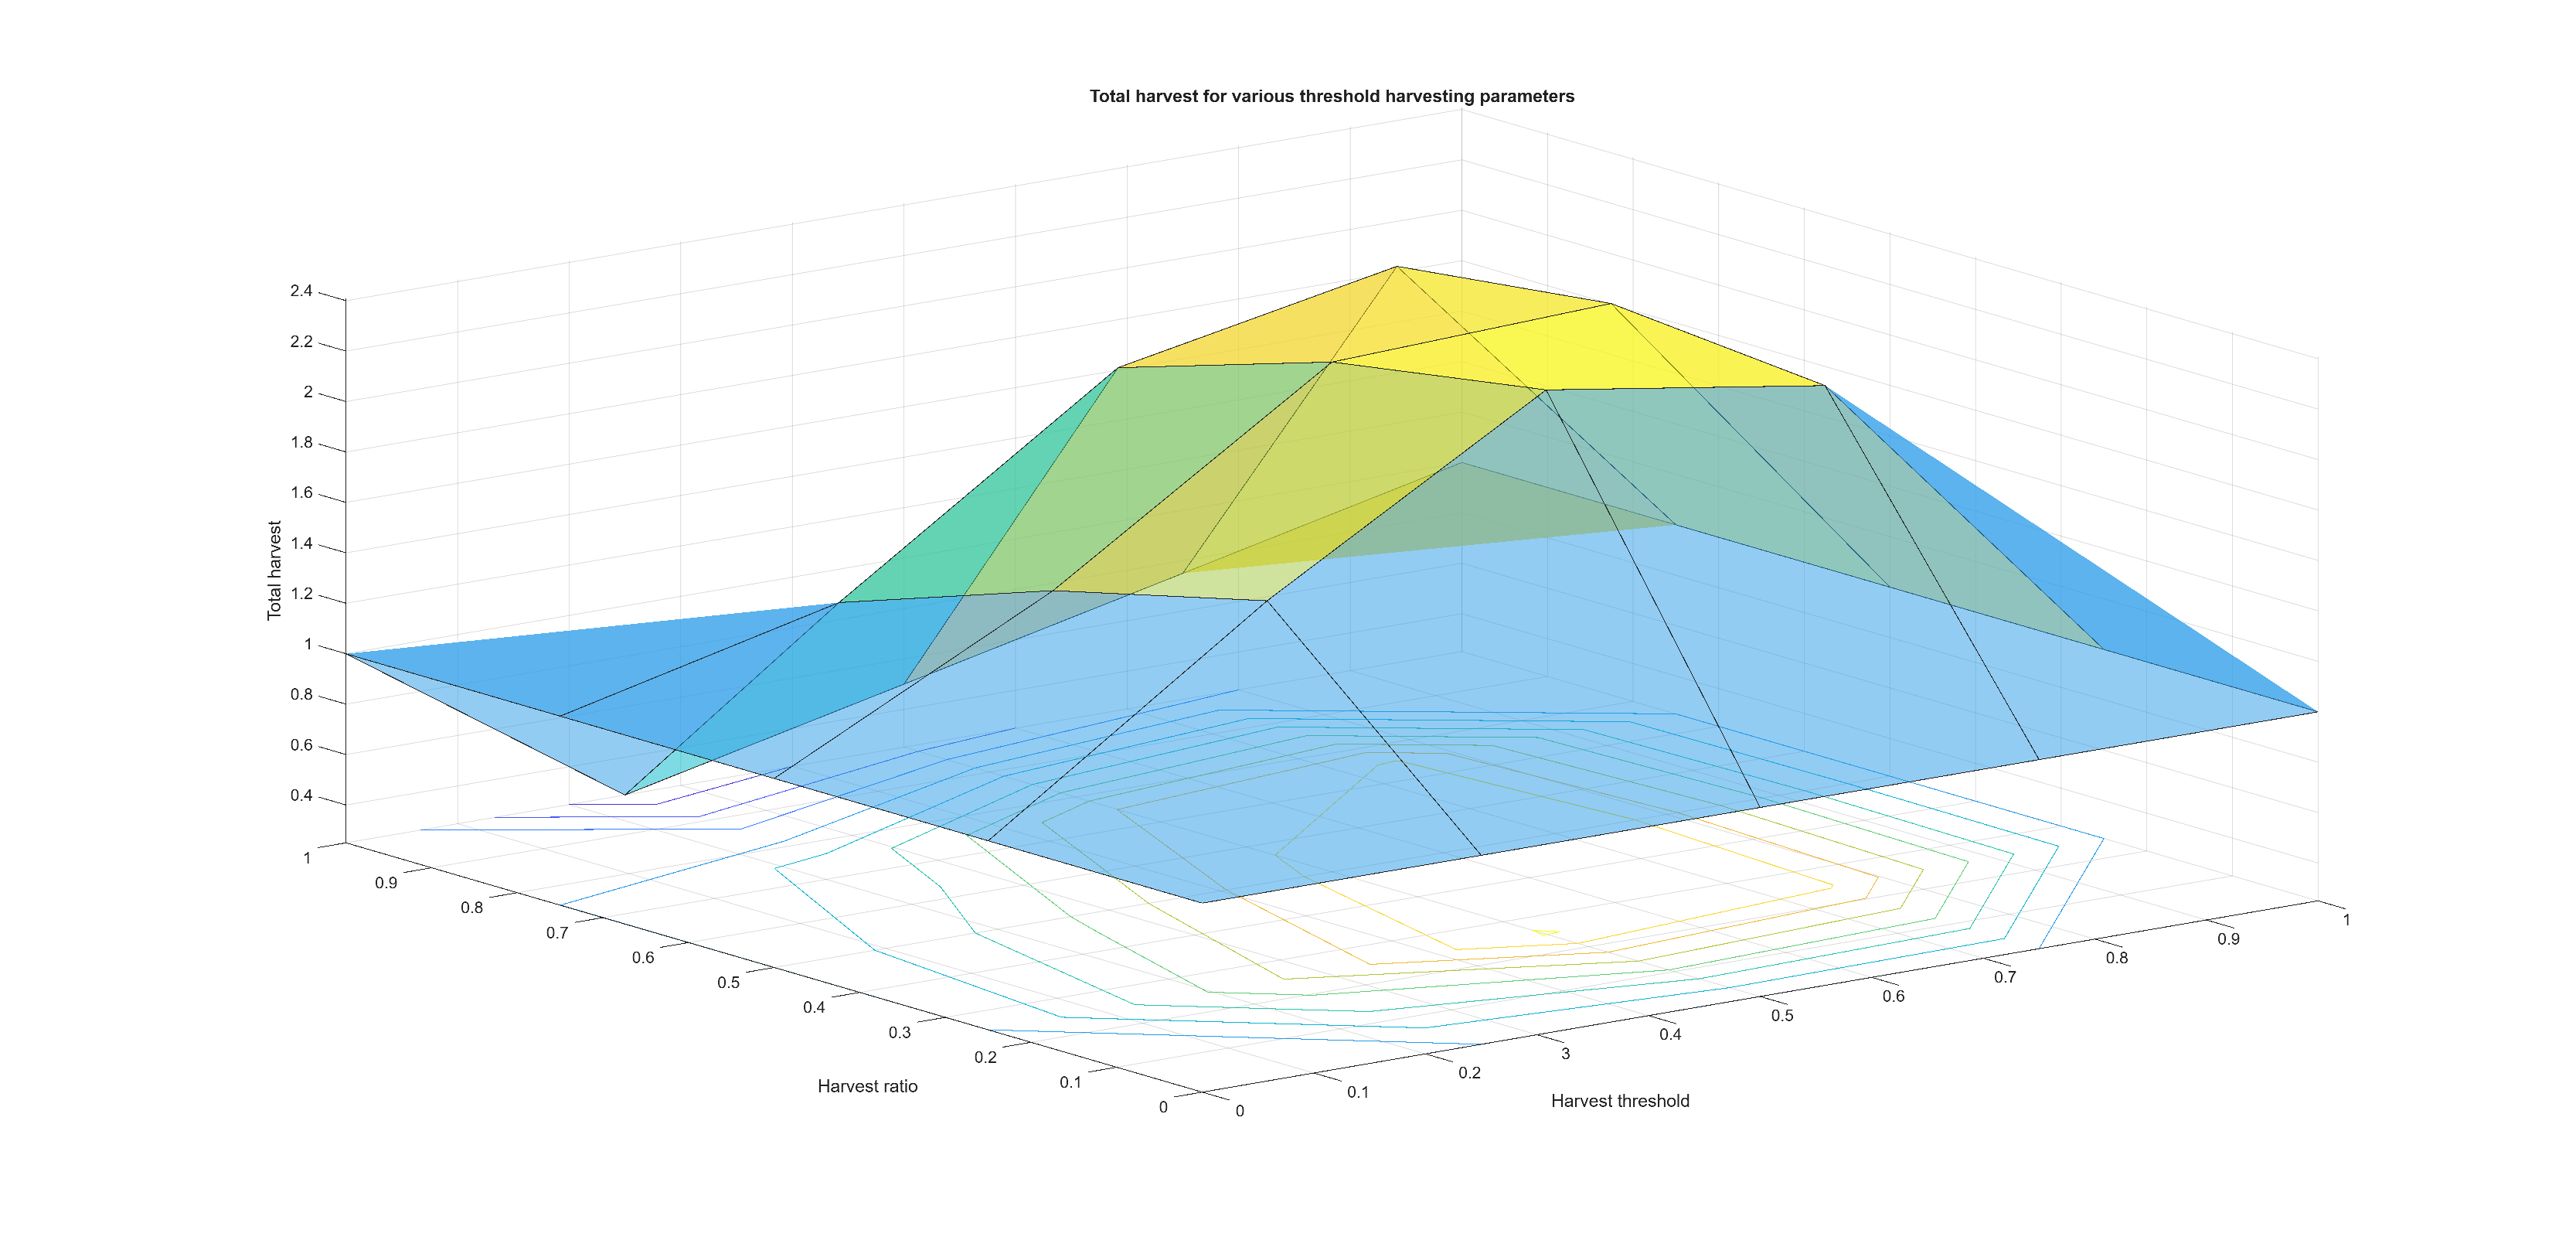
\includegraphics[width=\textwidth]{Plots/task4d}
        \caption{Objective function plot for subtask 4d)}
    \end{figure}

    \item The gradient of the objective function $F$ is given by
    \begin{equation}\label{eq:fish_gradient}
       \nabla F(T, \alpha) = \nabla P(5; T, \alpha) + \nabla H(5; T, \alpha) = (G_p)_{1,:}(5; T, \alpha) + (G_p)_{2,:}(5; T, \alpha)
    \end{equation}
    where $(G_p)_{i, :}(t; T, \alpha)$ denotes the i-th row of the parameter sensitivity matrix of the system given by \cref{eq:fish_harvest} and \cref{eq:fish_jump} with parameters $T$ and $\alpha$ at time point $t$. \\ \\
    \textbf{Subtask:} \\
    Compute the gradient of the objective function $\nabla F$ on a parameter grid using the solutions obtained from subtask \ref{item:task4c}.\\
    Plot the results. Where does the gradient point for the parameters which maximize $F$ on the grid? \\ \\
    \textbf{Steps:}
    \begin{enumerate}[label=\arabic*.]
       \item Implement the function \lstinline|g = computeGradient(datahandle, solution)| in the file \texttt{runTask4.m}, which should take a datahandle and solution and return the gradient of the objective function for the given solution as described \cref{eq:fish_gradient}.
       \item Use the provided code \lstinline|gradientFunc = @(solution) computeGradient(datahandle, solution)| to define an anonymous function, which takes a solution and returns the gradient.
       \item Use the provided code \lstinline|gradientGrid = arrayfun(gradientFunc, solutionGrid, 'UniformOutput', false)| to apply your gradient function to each solution in the grid.
       \item Use the provided function \lstinline|plotGradient(solutionGrid, objectiveGrid, gradientGrid)| to plot your gradients as arrows in a 3D surface plot of the objective function.
    \end{enumerate}
    \textbf{Hints:}
    \begin{itemize}
       \item Check the appendix for a reminder on how to compute sensitivities using IFDIFF.
       \item We only need the sensitivity at the integration time interval end point, which can be obtained using \lstinline|solution.x(end)|.
       \item Since the sensitivity is only computed for one time point, you can obtain the parameter sensitivity matrix directly from the sensitivity output struct using \lstinline|sens.Gp|.
       \item Since we only need the parameter sensitivities and not the initial value sensitivities, you can pass the optional flag \lstinline|generateSensitivityFunction(..., 'calcGy', false)| to prevent unnecessary computations.
    \end{itemize}
    \textbf{Reference plot:}
    \begin{figure}[H]
        \centering
        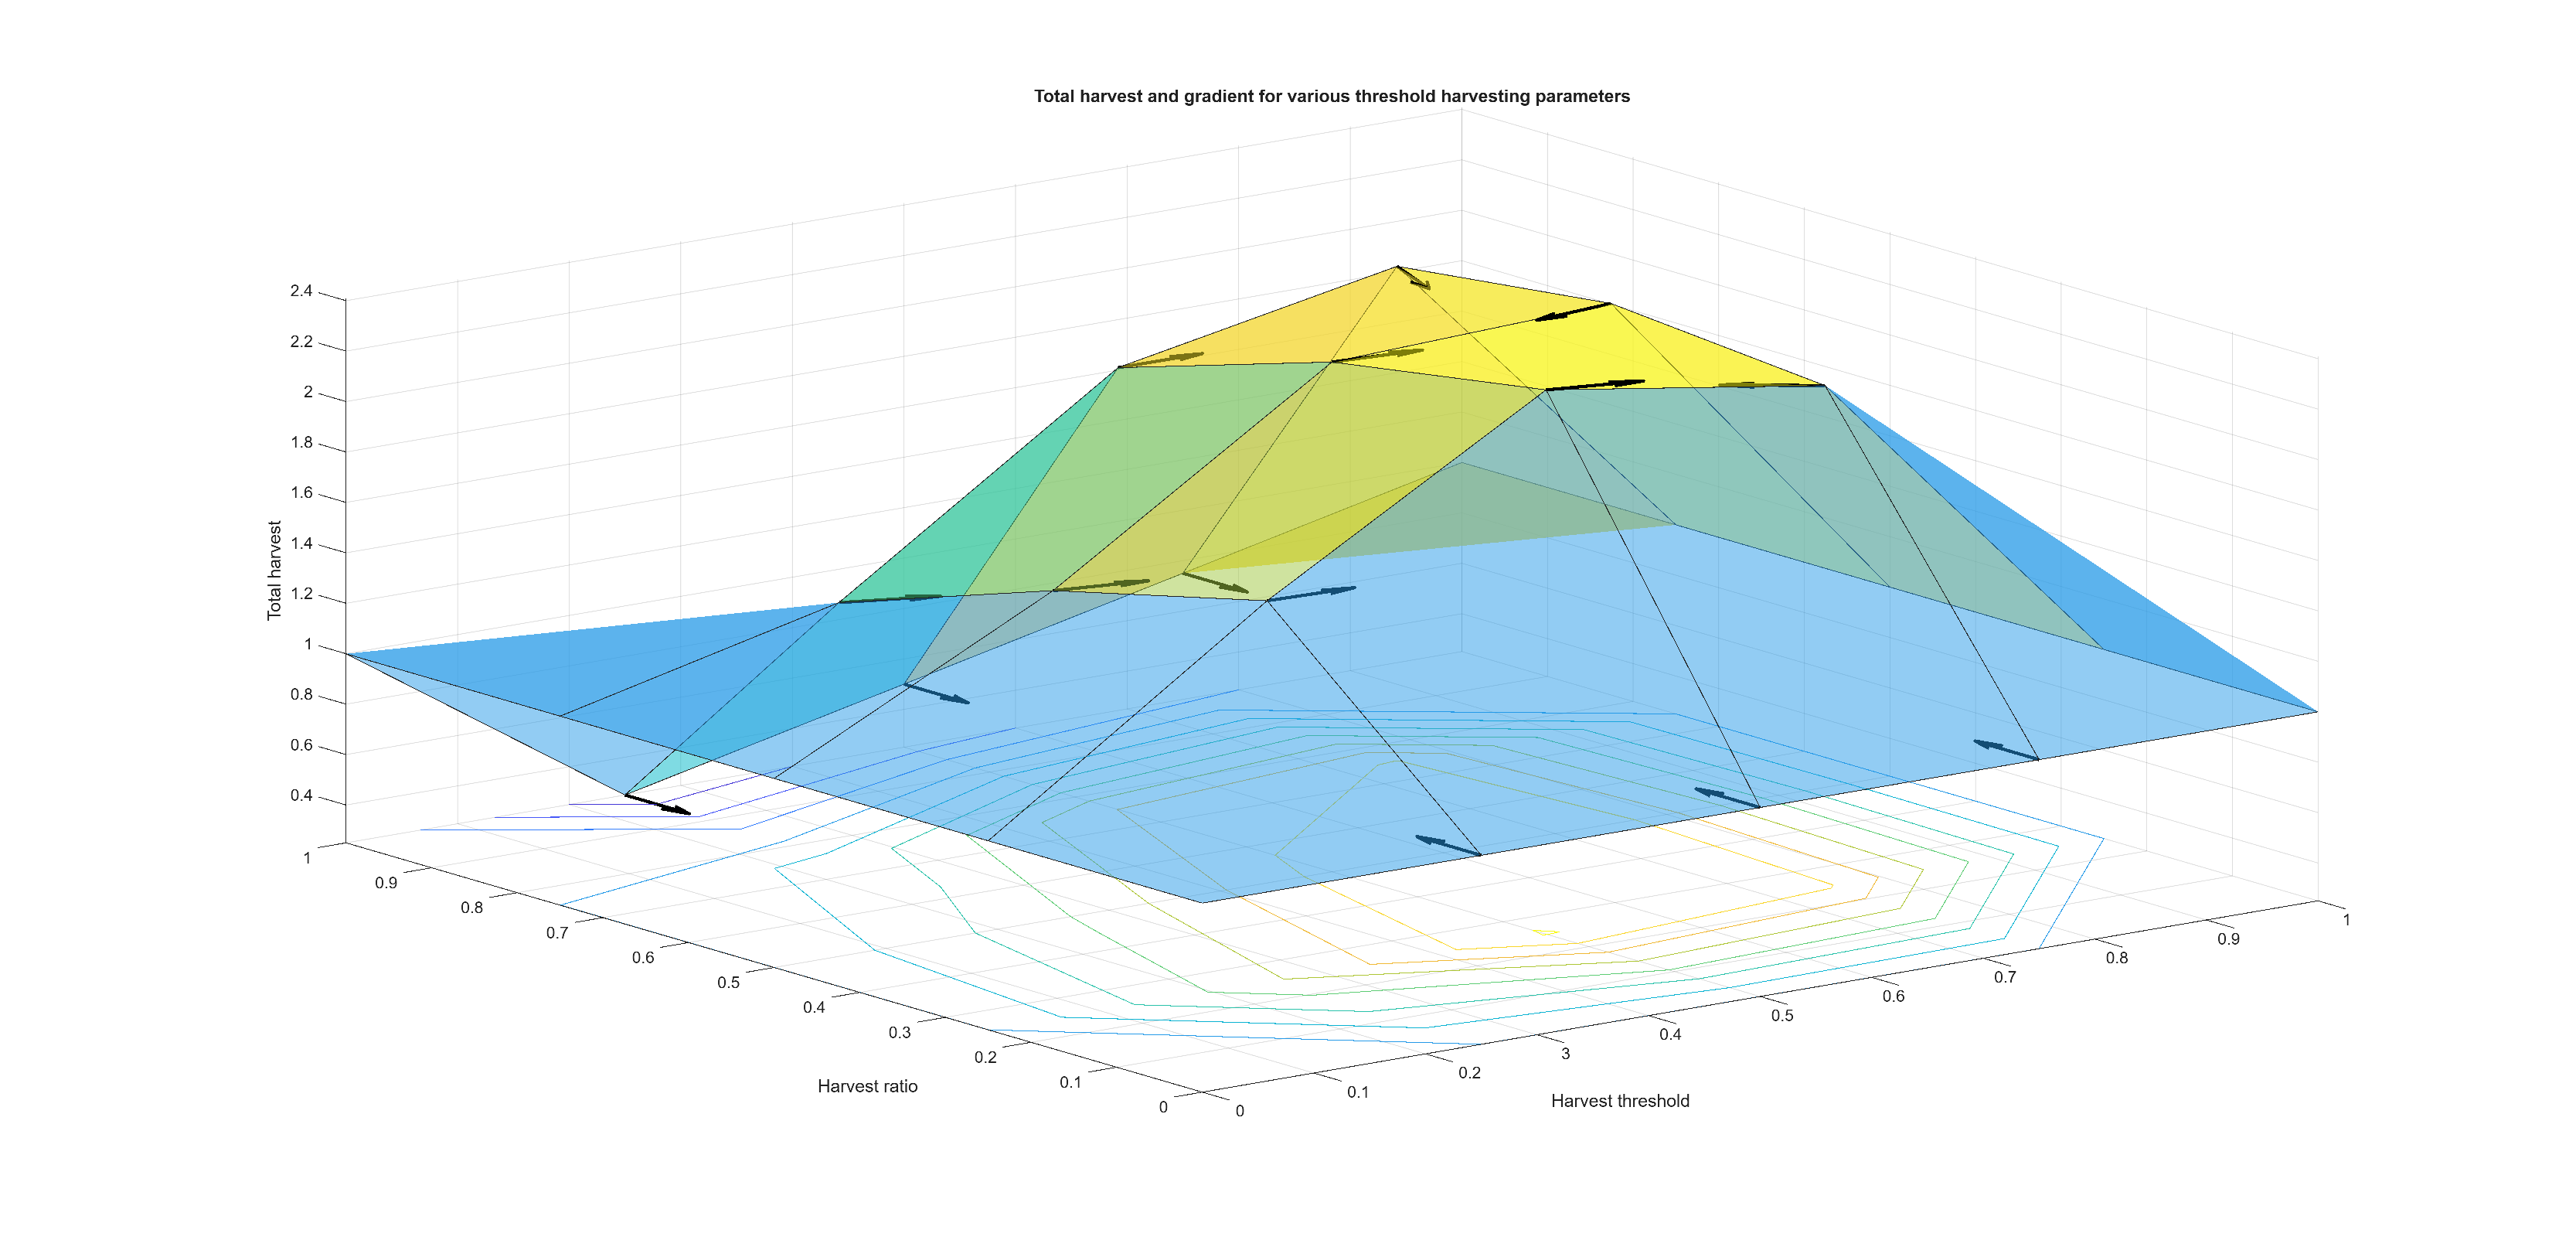
\includegraphics[width=\textwidth]{Plots/task4e}
        \caption{Gradient plot for subtask 4e)}
    \end{figure}

    \item After computing the gradients, we can now optimize the parameters $T$ and $\alpha$ in order to maximize the total amount of fish produced as described by the objective function $F$. However, we will additionaly impose a lower bound constraint on the harvest ratio, namely $\alpha \geq 0.2$, because the number of state jumps approaches infinity as $\alpha$ goes towards zero, which would make the problem ill-posed (Zeno behavior).
     
    The optimal parameters $T^*$ and $\alpha^*$ are then defined via
    \begin{equation}\label{eq:fish_optim}
       F(T^*, \alpha^*) = \max_{T \in [0, C], \alpha \in [0.2, 1]} F(T, \alpha)
    \end{equation}
    \textbf{Subtask:} \\
    Use MATLAB's optimizer \lstinline|fmincon| to compute the optimal parameters $T^*$ and $\alpha^*$ which maximize the objective function $F$ as described in \cref{eq:fish_optim}. \\
    Use IFDIFF to compute the solution for the optimal parameters and plot the result. What are the maximum and minimum values of the population after the first harvest? Which point lies exactly between the maximum and minimum values? Can you explain intuitively why the midpoint has to lie where it does for the optimal parameters? Think back to the solution without state jumps. When is the population growth maximized? \\ \\
    \textbf{Steps:}
    \begin{enumerate}[label=\arabic*.]
        \item Implement the function \lstinline|[f, g] = objWithGrad(p, solutionFunc, objectiveFunc, gradientFunc)| in the file \texttt{runTask4.m}. The function should take a parameter vector and the solution, objective and gradient functions that you have implemented in the previous subtasks and return the \textit{negative} objective \lstinline|f| and gradient \lstinline|g| for the given parameters. It is crucial that the objective and gradient are negated because MATLAB optimizers can only handle minimization problems, so we need to flip the signs of our objective and gradient to transform our maximization problem into an equivalent minimization problem.
        \item Use the provided code \lstinline|optimizationFunc = @(p) objWithGrad(p, solutionFunc, objectiveFunc, gradientFunc)| to define an anonymous function which takes a parameter vector and returns the negated objective and gradient.
        \item Use the provided function \lstinline|[pOpt, objOpt] = optimizeParameters(optimizationFunc)| to setup the optimization problem and compute the optimal parameters and objective value using \lstinline|fmincon|.
        \item Compute the solution for the optimal parameters using the function \lstinline|solutionFunc| from subtask \ref{item:task4c}.
        \item Use the provided function \lstinline|plotPopulation(solutionOpt)| to plot the solution for the optimal parameters.
    \end{enumerate}
    \textbf{Hints:}
    \begin{itemize}
        \item Remember that \lstinline|solutionFunc| takes a parameter and returns a solution, whereas \lstinline|objectiveFunc| and \lstinline|gradientFunc| take a solution and return the objective and gradient.
        \item Don't forget to negate your objective and gradient in the function \lstinline|objWithGrad|.
    \end{itemize}
    \textbf{Reference plot:}
    \begin{figure}[H]
        \centering
        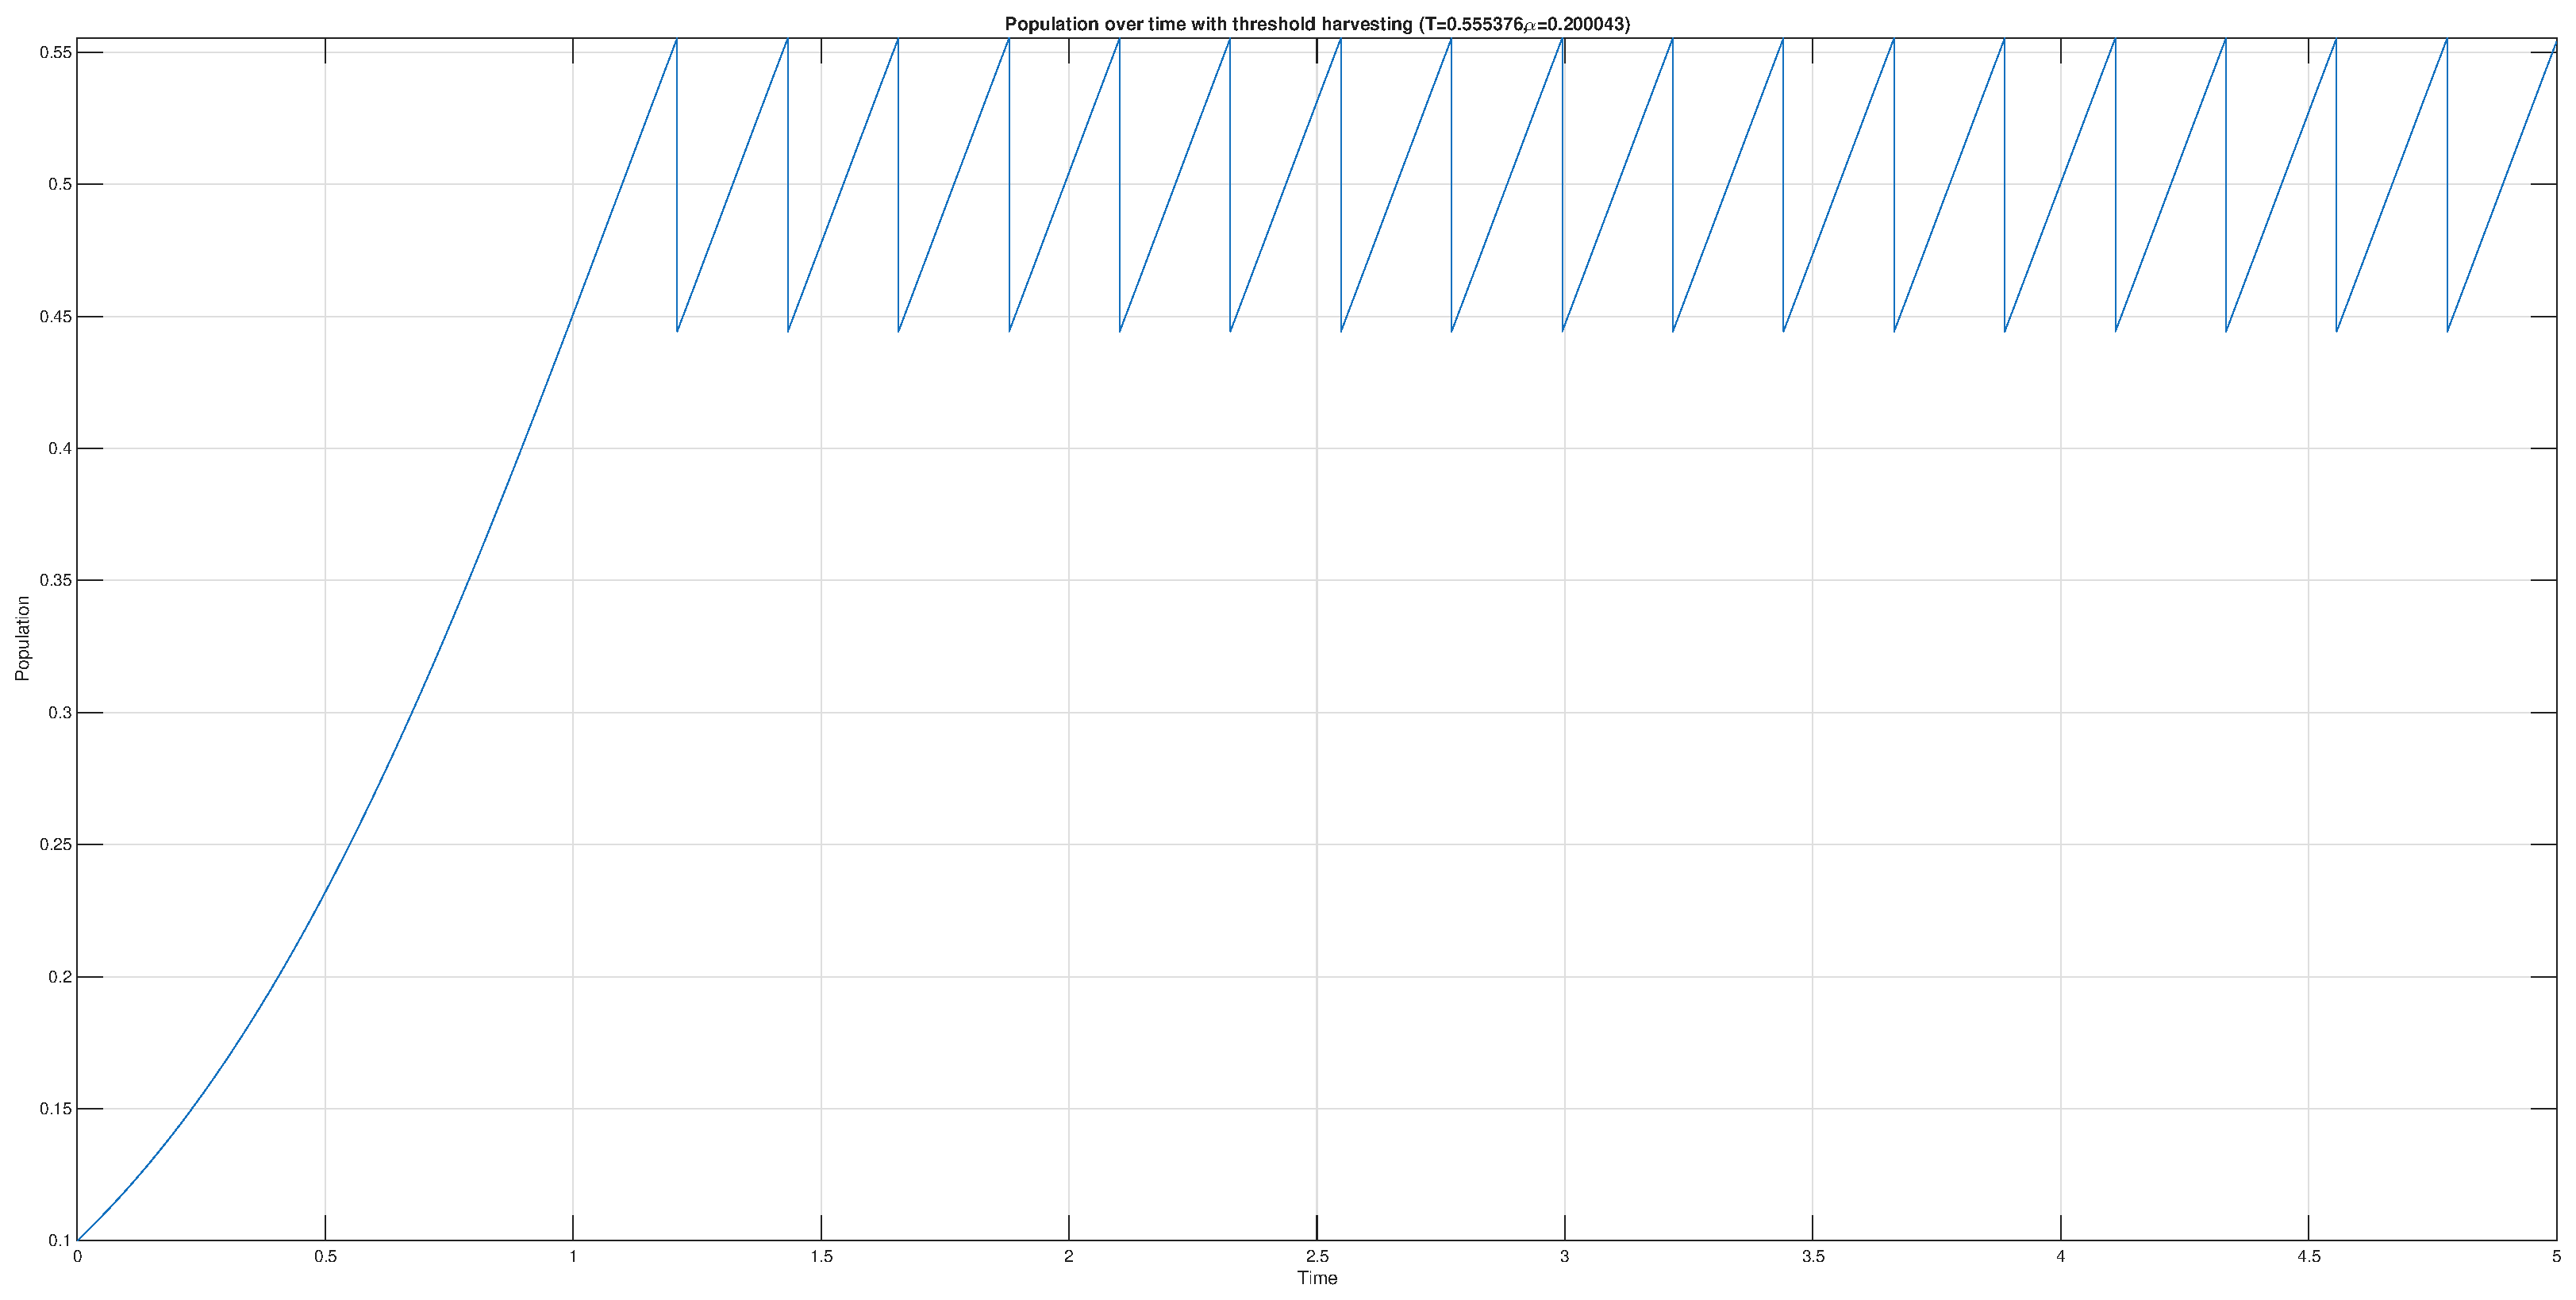
\includegraphics[width=\textwidth]{Plots/task4f}
        \caption{Optimized population plot for subtask 4f)}
    \end{figure}
\end{enumerate}
